\documentclass{standalone}
\usepackage{tikz}
\usepackage{pgfplots}
\pgfplotsset{compat=newest}
\usepackage{amsmath}
\usepackage[american]{circuitikz}
\usepackage{cmbright}

\ctikzset{bipoles/resistor/height=0.2, bipoles/resistor/width=0.6}

\definecolor{myred}{RGB}{170,0,0}
\definecolor{myblue}{RGB}{0,0,220}
\definecolor{mygreen}{RGB}{0,150,0}
\definecolor{myorange}{RGB}{255,127,0}
\definecolor{mybrown}{RGB}{150,75,0}

\begin{document}
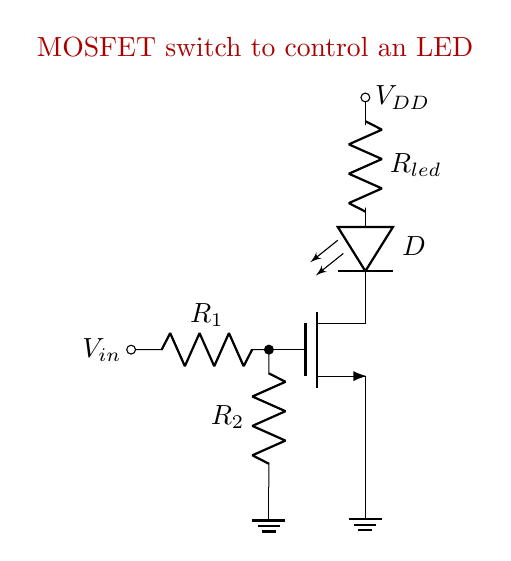
\begin{tikzpicture}
    \begin{scope}[scale=0.7]
        % Title
        \node[anchor=center, color=myred] at (-2.0, 2.5) {MOSFET switch to control an LED};
        
        \draw (0, -3) node[nmos, scale=1.25] (Q) {};
        \draw (Q.gate) 
            to[R, l_={$R_1$}] ++(-2.25, 0)
            to[short, -o] ++(-0.25, 0)
            node[anchor=east, align=center] {$V_{in}$};
        \draw (Q.gate)
            to[R, *-, l_={$R_2$}] ++(0, -2.5)
            node[ground] {};
        \draw (Q.source)
            to[short] ++(0, -1.1)
            node[ground] {};
        \draw[-Latex, thin] ($(Q.source) + (-0.6, 0.895)$) -- ++(0.625, 0);
        \draw ($(Q.drain) + (0, -0.3)$)
            to[led, l_=$D$, invert] + +(0, 1.5)
            to[R, l_={$R_{led}$}] ++(0, 1.5)
            to[short, -o] ++(0, 0.5)
            node[anchor=west, align=center] {$V_{DD}$};
    \end{scope}
\end{tikzpicture}
\end{document}